% file: 2-11-heapsort/heap-decreasing-order-7.tex
% 7: containing 7 nodes

\documentclass[tikz]{standalone}
\usepackage{tikz-qtree}

\begin{document}
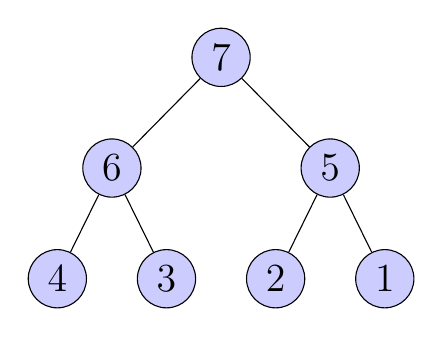
\begin{tikzpicture} [level distance = 40pt, sibling distance = 18pt,
  edge from parent/.style= { % added code
      draw, edge from parent path = {(\tikzparentnode) -- (\tikzchildnode)}}]
  \tikzset{every tree node/.style = 
    {align = center, circle, draw, fill = blue!20, font = \Large}}
    \Tree [.$7$
	    [.$6$
	       $4$ 
	       $3$
            ]
	    [.$5$ 
	      $2$
	      $1$
	   ] 
        ]
\end{tikzpicture}
\end{document}
